\documentclass{anstrans}
%%%%%%%%%%%%%%%%%%%%%%%%%%%%%%%%%%%
\title{Full-core analysis of thorium-fueled Molten Salt Breeder Reactor using 
the SERPENT 2 Monte Carlo code}

\author{Andrei Rykhlevskii, Alexander Lindsay, Kathryn Huff}

\institute{
Department of Nuclear, Plasma, and Radiological Engineering, University of 
Illinois at Urbana-Champaign \break
Urbana, IL
}

\email{andreir2@illinois.edu}

%%%% packages and definitions (optional)
\usepackage{graphicx} % allows inclusion of graphics
\usepackage{caption}  % allows center figures caption
\usepackage{booktabs} % nice rules (thick lines) for tables
\usepackage{microtype} % improves typography for PDF
\usepackage[section]{placeins}
\usepackage[acronym,toc]{glossaries}  % acronyms inclusion

%\newacronym{<++>}{<++>}{<++>}
\newacronym[longplural={metric tons of heavy metal}]{MTHM}{MTHM}{metric ton of heavy metal}
\newacronym{ABM}{ABM}{agent-based modeling}
\newacronym{ACDIS}{ACDIS}{Program in Arms Control \& Domestic and International Security}
\newacronym{AHTR}{AHTR}{Advanced High Temperature Reactor}
\newacronym{ANDRA}{ANDRA}{Agence Nationale pour la gestion des D\'echets RAdioactifs, the French National Agency for Radioactive Waste Management}
\newacronym{ANL}{ANL}{Argonne National Laboratory}
\newacronym{API}{API}{application programming interface}
\newacronym{ARCH}{ARCH}{autoregressive conditional heteroskedastic}
\newacronym{ARE}{ARE}{Aircraft Reactor Experiment}
\newacronym{ARFC}{ARFC}{Advanced Reactors and Fuel Cycles}
\newacronym{ARMA}{ARMA}{autoregressive moving average}
\newacronym{ASME}{ASME}{American Society of Mechanical Engineers}
\newacronym{ATWS}{ATWS}{Anticipated Transient Without Scram}
\newacronym{BDBE}{BDBE}{Beyond Design Basis Event}
\newacronym{BIDS}{BIDS}{Berkeley Institute for Data Science}
\newacronym{BOL}{BOL}{Beginning-of-Life}
\newacronym{BSD}{BSD}{Berkeley Software Distribution}
\newacronym{CAFCA}{CAFCA}{Code for Advanced Fuel Cycles Assessment}
\newacronym{CASL}{CASL}{Consortium for Advanced Simulation of Light Water Reactors}
\newacronym{CDTN}{CDTN}{Centro de Desenvolvimento da Tecnologia Nuclear}
\newacronym{CEA}{CEA}{Commissariat \`a l'\'Energie Atomique et aux \'Energies Alternatives}
\newacronym{CFD}{CFD}{Computational Fluid Dynamics}
\newacronym{CG}{CG}{Continuous Galerkin}
\newacronym{CI}{CI}{continuous integration}
\newacronym{CNEN}{CNEN}{Comiss\~{a}o Nacional de Energia Nuclear}
\newacronym{CNERG}{CNERG}{Computational Nuclear Engineering Research Group}
\newacronym{COMSOL}{COMSOL}{COMmon SOLution}
\newacronym{COSI}{COSI}{Commelini-Sicard}
\newacronym{COTS}{COTS}{commercial, off-the-shelf}
\newacronym{CSNF}{CSNF}{commercial spent nuclear fuel}
\newacronym{CTAH}{CTAHs}{Coiled Tube Air Heaters}
\newacronym{CUBIT}{CUBIT}{CUBIT Geometry and Mesh Generation Toolkit}
\newacronym{CURIE}{CURIE}{Centralized Used Fuel Resource for Information Exchange}
\newacronym{DAG}{DAG}{directed acyclic graph}
\newacronym{DANESS}{DANESS}{Dynamic Analysis of Nuclear Energy System Strategies}
\newacronym{DBE}{DBE}{Design Basis Event}
\newacronym{DESAE}{DESAE}{Dynamic Analysis of Nuclear Energy Systems Strategies}
\newacronym{DG}{DG}{Discontinuous Galerkin}
\newacronym{DHS}{DHS}{Department of Homeland Security}
\newacronym{DOE}{DOE}{Department of Energy}
\newacronym{DRACS}{DRACS}{Direct Reactor Auxiliary Cooling System}
\newacronym{DRE}{DRE}{dynamic resource exchange}
\newacronym{DSNF}{DSNF}{DOE spent nuclear fuel}
\newacronym{DYMOND}{DYMOND}{Dynamic Model of Nuclear Development }
\newacronym{EBS}{EBS}{Engineered Barrier System}
\newacronym{EDZ}{EDZ}{Excavation Disturbed Zone}
\newacronym{EIA}{EIA}{U.S. Energy Information Administration}
\newacronym{EPA}{EPA}{Environmental Protection Agency}
\newacronym{EP}{EP}{Engineering Physics}
\newacronym{FCO}{FCO}{Fuel Cycle Options}
\newacronym{FCT}{FCT}{Fuel Cycle Technology}
\newacronym{FEHM}{FEHM}{Finite Element Heat and Mass Transfer}
\newacronym{FEPs}{FEPs}{Features, Events, and Processes}
\newacronym{FHR}{FHR}{Fluoride-Salt-Cooled High-Temperature Reactor}
\newacronym{FLiBe}{FLiBe}{Fluoride-Lithium-Beryllium}
\newacronym{GCAM}{GCAM}{Global Change Assessment Model}
\newacronym{GDSE}{GDSE}{Generic Disposal System Environment}
\newacronym{GDSM}{GDSM}{Generic Disposal System Model}
\newacronym{GENIUSv1}{GENIUSv1}{Global Evaluation of Nuclear Infrastructure Utilization Scenarios, Version 1}
\newacronym{GENIUSv2}{GENIUSv2}{Global Evaluation of Nuclear Infrastructure Utilization Scenarios, Version 2}
\newacronym{GENIUS}{GENIUS}{Global Evaluation of Nuclear Infrastructure Utilization Scenarios}
\newacronym{GPAM}{GPAM}{Generic Performance Assessment Model}
\newacronym{GRSAC}{GRSAC}{Graphite Reactor Severe Accident Code}
\newacronym{GUI}{GUI}{graphical user interface}
\newacronym{HLW}{HLW}{high level waste}
\newacronym{HPC}{HPC}{high-performance computing}
\newacronym{HTC}{HTC}{high-throughput computing}
\newacronym{HTGR}{HTGR}{High Temperature Gas-Cooled Reactor}
\newacronym{IAEA}{IAEA}{International Atomic Energy Agency}
\newacronym{IEMA}{IEMA}{Illinois Emergency Mangament Agency}
\newacronym{INL}{INL}{Idaho National Laboratory}
\newacronym{IPRR1}{IRP-R1}{Instituto de Pesquisas Radioativas Reator 1}
\newacronym{IRP}{IRP}{Integrated Research Project}
\newacronym{ISFSI}{ISFSI}{Independent Spent Fuel Storage Installation}
\newacronym{ISRG}{ISRG}{Independent Student Research Group}
\newacronym{JFNK}{JFNK}{Jacobian-Free Newton Krylov}
\newacronym{LANL}{LANL}{Los Alamos National Laboratory}
\newacronym{LBNL}{LBNL}{Lawrence Berkeley National Laboratory}
\newacronym{LCOE}{LCOE}{levelized cost of electricity}
\newacronym{LDRD}{LDRD}{laboratory directed research and development}
\newacronym{LFR}{LFR}{Lead-Cooled Fast Reactor}
\newacronym{LGPL}{LGPL}{Lesser GNU Public License}
\newacronym{LLNL}{LLNL}{Lawrence Livermore National Laboratory}
\newacronym{LMFBR}{LMFBR}{Liquid-Metal-cooled Fast Breeder Reactor}
\newacronym{LOFC}{LOFC}{Loss of Forced Cooling}
\newacronym{LOHS}{LOHS}{Loss of Heat Sink}
\newacronym{LOLA}{LOLA}{Loss of Large Area}
\newacronym{LP}{LP}{linear program}
\newacronym{LWR}{LWR}{Light Water Reactor}
\newacronym{MARKAL}{MARKAL}{MARKet and ALlocation}
\newacronym{MA}{MA}{minor actinide}
\newacronym{MCNP}{MCNP}{Monte Carlo N-Particle code}
\newacronym{MILP}{MILP}{mixed-integer linear program}
\newacronym{MIT}{MIT}{the Massachusetts Institute of Technology}
\newacronym{MOAB}{MOAB}{Mesh-Oriented datABase}
\newacronym{MOOSE}{MOOSE}{Multiphysics Object-Oriented Simulation Environment}
\newacronym{MOX}{MOX}{mixed oxide}
\newacronym{MPI}{MPI}{Message Passing Interface}
\newacronym{MSBR}{MSBR}{Molten Salt Breeder Reactor}
\newacronym{MSFR}{MSFR}{Molten Salt Fast Reactor}
\newacronym{MSRE}{MSRE}{Molten Salt Reactor Experiment}
\newacronym{MSR}{MSR}{Molten Salt Reactor}
\newacronym{NAGRA}{NAGRA}{National Cooperative for the Disposal of Radioactive Waste}
\newacronym{NCSA}{NCSA}{National Center for Supercomputing Applications}
\newacronym{NEAMS}{NEAMS}{Nuclear Engineering Advanced Modeling and Simulation}
\newacronym{NEUP}{NEUP}{Nuclear Energy University Programs}
\newacronym{NFCSim}{NFCSim}{Nuclear Fuel Cycle Simulator}
\newacronym{NFC}{NFC}{Nuclear Fuel Cycle}
\newacronym{NGNP}{NGNP}{Next Generation Nuclear Plant}
\newacronym{NMWPC}{NMWPC}{Nuclear MW Per Capita}
\newacronym{NNSA}{NNSA}{National Nuclear Security Administration}
\newacronym{NPRE}{NPRE}{Department of Nuclear, Plasma, and Radiological Engineering}
\newacronym{NQA1}{NQA-1}{Nuclear Quality Assurance - 1}
\newacronym{NRC}{NRC}{Nuclear Regulatory Commission}
\newacronym{NSF}{NSF}{National Science Foundation}
\newacronym{NSSC}{NSSC}{Nuclear Science and Security Consortium}
\newacronym{NUWASTE}{NUWASTE}{Nuclear Waste Assessment System for Technical Evaluation}
\newacronym{NWF}{NWF}{Nuclear Waste Fund}
\newacronym{NWTRB}{NWTRB}{Nuclear Waste Technical Review Board}
\newacronym{OCRWM}{OCRWM}{Office of Civilian Radioactive Waste Management}
\newacronym{ORION}{ORION}{ORION}
\newacronym{ORNL}{ORNL}{Oak Ridge National Laboratory}
\newacronym{PARCS}{PARCS}{Purdue Advanced Reactor Core Simulator}
\newacronym{PBAHTR}{PB-AHTR}{Pebble Bed Advanced High Temperature Reactor}
\newacronym{PBFHR}{PB-FHR}{Pebble-Bed Fluoride-Salt-Cooled High-Temperature Reactor}
\newacronym{PEI}{PEI}{Peak Environmental Impact}
\newacronym{PH}{PRONGHORN}{PRONGHORN}
\newacronym{PRKE}{PRKE}{Point Reactor Kinetics Equations}
\newacronym{PSPG}{PSPG}{Pressure-Stabilizing/Petrov-Galerkin}
\newacronym{PWAR}{PWAR}{Pratt and Whitney Aircraft Reactor}
\newacronym{PWR}{PWR}{Pressurized Water Reactor}
\newacronym{PetSc}{PetSc}{Portable, Extensible Toolkit for Scientific Computation}
\newacronym{PyNE}{PyNE}{Python toolkit for Nuclear Engineering}
\newacronym{PyRK}{PyRK}{Python for Reactor Kinetics}
\newacronym{QA}{QA}{quality assurance}
\newacronym{RDD}{RD\&D}{Research Development and Demonstration}
\newacronym{RD}{R\&D}{Research and Development}
\newacronym{RELAP}{RELAP}{Reactor Excursion and Leak Analysis Program}
\newacronym{RIA}{RIA}{Reactivity Insertion Accident}
\newacronym{RIF}{RIF}{Region-Institution-Facility}
\newacronym{SFR}{SFR}{Sodium-Cooled Fast Reactor}
\newacronym{SINDAG}{SINDA{\textbackslash}G}{Systems Improved Numerical Differencing Analyzer $\backslash$ Gaski}
\newacronym{SKB}{SKB}{Svensk K\"{a}rnbr\"{a}nslehantering AB}
\newacronym{SNF}{SNF}{spent nuclear fuel}
\newacronym{SNL}{SNL}{Sandia National Laboratory}
\newacronym{STC}{STC}{specific temperature change}
\newacronym{SUPG}{SUPG}{Streamline-Upwind/Petrov-Galerkin}
\newacronym{SWF}{SWF}{Separations and Waste Forms}
\newacronym{SWU}{SWU}{Separative Work Unit}
\newacronym{TRIGA}{TRIGA}{Training Research Isotope General Atomic}
\newacronym{TRISO}{TRISO}{Tristructural Isotropic}
\newacronym{TSM}{TSM}{Total System Model}
\newacronym{TSPA}{TSPA}{Total System Performance Assessment for the Yucca Mountain License Application}
\newacronym{ThOX}{ThOX}{thorium oxide}
\newacronym{UFD}{UFD}{Used Fuel Disposition}
\newacronym{UML}{UML}{Unified Modeling Language}
\newacronym{UOX}{UOX}{uranium oxide}
\newacronym{UQ}{UQ}{uncertainty quantification}
\newacronym{US}{US}{United States}
\newacronym{UW}{UW}{University of Wisconsin}
\newacronym{VISION}{VISION}{the Verifiable Fuel Cycle Simulation Model}
\newacronym{VV}{V\&V}{verification and validation}
\newacronym{WIPP}{WIPP}{Waste Isolation Pilot Plant}
\newacronym{YMR}{YMR}{Yucca Mountain Repository Site}
\newacronym{gpm}{gpm}{gallons per minute}

\graphicspath{{figures/}}
\captionsetup{justification   = raggedright,
              singlelinecheck = false}
\newcommand{\SN}{S$_N$}
\renewcommand{\vec}[1]{\bm{#1}} %vector is bold italic
\newcommand{\vd}{\bm{\cdot}} % slightly bold vector dot
\newcommand{\grad}{\vec{\nabla}} % gradient
\newcommand{\ud}{\mathop{}\!\mathrm{d}} % upright derivative symbol
\makeglossaries

\begin{document}
%%%%%%%%%%%%%%%%%%%%%%%%%%%%%%%%%%%%%%%%%%%%%%%%%%%%%%%%%%%%%%%%%%%%%%%%%%%%%%%%
\section{Introduction}
The \gls{MSR} is an advanced type of reactor which was developed at \gls{ORNL} 
in the 1950s and was operated in the 1960s. In the MSR, fluorides of fissile 
and/or fertile materials (i.e. UF$_4$, PuF$_3$ and/or ThF$_4$) are mixed with 
carrier salts to form a liquid fuel which is circulated in a loop-type primary 
circuit \cite{haubenreich_experience_1970}. This innovation leads to immediate 
advantages over traditional, solid-fueled, reactors. These include 
near-atmospheric pressure in the primary loop, relatively high coolant 
temperature, outstanding neutron economy, a high level of inherent safety, 
reduced fuel preprocessing, and the ability to continuously remove fission 
products and add fissile and/or fertile elements \cite{leblanc_molten_2010}. 

The thermal spectrum \gls{MSBR} was designed to realize the promise of the 
thorium fuel cycle, which uses of natural thorium instead of enriched uranium.  
Thorium breeds fissile $^{233}$U and avoids uranium enrichment. The mixture of 
LiF-BeF$_2$-ThF$_4$-UF$_4$-PuF$_3$ has a melting point of $499^\circ$C, a low 
vapor pressure at operating temperatures, and good flow and heat transfer 
properties \cite{robertson_conceptual_1971}. The \gls{MSBR} complex geometry is 
challenging to describe in software input and usually require major geometric 
approximations \cite{park_whole_2015}. 

We used the continuous-energy Serpent 2 Monte Carlo particle transport code to 
calulate whole-core depletion in the \gls{MSBR}. We then compare these results 
with existing MCNP6 results with a more simplified geometric model 
\cite{park_whole_2015,leppanen_serpent_2012}. This neutronics model is of 
sufficient fidelity to inform optimization of fuel salt composition, fuel 
utilization, neutron fluxes, and spectrum evaluation. Moreover, this model  
will be employed for depeletion calculations, generation of problem-oriented 
homogenized nuclear data (multi-group cross sections and diffusion constants) 
for deterministic reactor codes, and multi-physics simulations 
\cite{fridman_use_2011,valtavirta_coupled_2017}.

All calculations presented in this paper were performed using Serpent 2 version 
2.1.28. Serpent 2 levereges hybrid OpenMP + MPI parallelized memory management, 
which enabled us to conduct depletion calculations on computer clusters with 
multiple cores \cite{leppanen_serpent_2015}. 

In Section 2, a brief description of the \gls{MSBR} geometry model is given. In 
Section 3 the results are presented and discussed. Section 4 reflects 
conclusions and plans for future research.  

%%%%%%%%%%%%%%%%%%%%%%%%%%%%%%%%%%%%%%%%%%%%%%%%%%%%%%%%%%%%%%%%%%%%%%%%%%%%%%%%
\section{MSBR design description}
The \gls{MSBR} vessel has diameter of 680 cm and a height of 610 cm. It 
contains a molten fluoride fuel-salt mixture that generates heat in the active 
core region and transports that heat to the primary heat exchanger by way of 
the primary salt pump.
In the active core region, the salt flows through channels in moderating and 
reflecting graphite blocks.

The core has two radial zones bounded by a solid cylindrical graphite reflector 
and the vessel wall.  Zones I and II are surrounded radially and axially by 
fuel salt. This space for fuel is necessary for injection and flow of molten 
salt.

Fig.~\ref{fig:plan} shows the plan view of the whole-core configuration at the 
expected reactor operational level when both graphite control rods are fully 
inserted, and the safety rods are fully withdrawn. The safety rods only get 
inserted during an accident.  

Fig.~\ref{fig:elevation} shows the longitudinal section of the reactor. The 
violet color represents bare graphite, and the yellow represents fuel salt. The 
blue color shows Hastelloy-N, a material used for the plenum and vessel wall, 
and the black color is a void space. In this work, all figures of the core were 
generated using the built-in Serpent plotter.

\begin{figure}[hbp!] % replace 't' with 'b' to 
  \centering
  \vspace{-0.3em}
  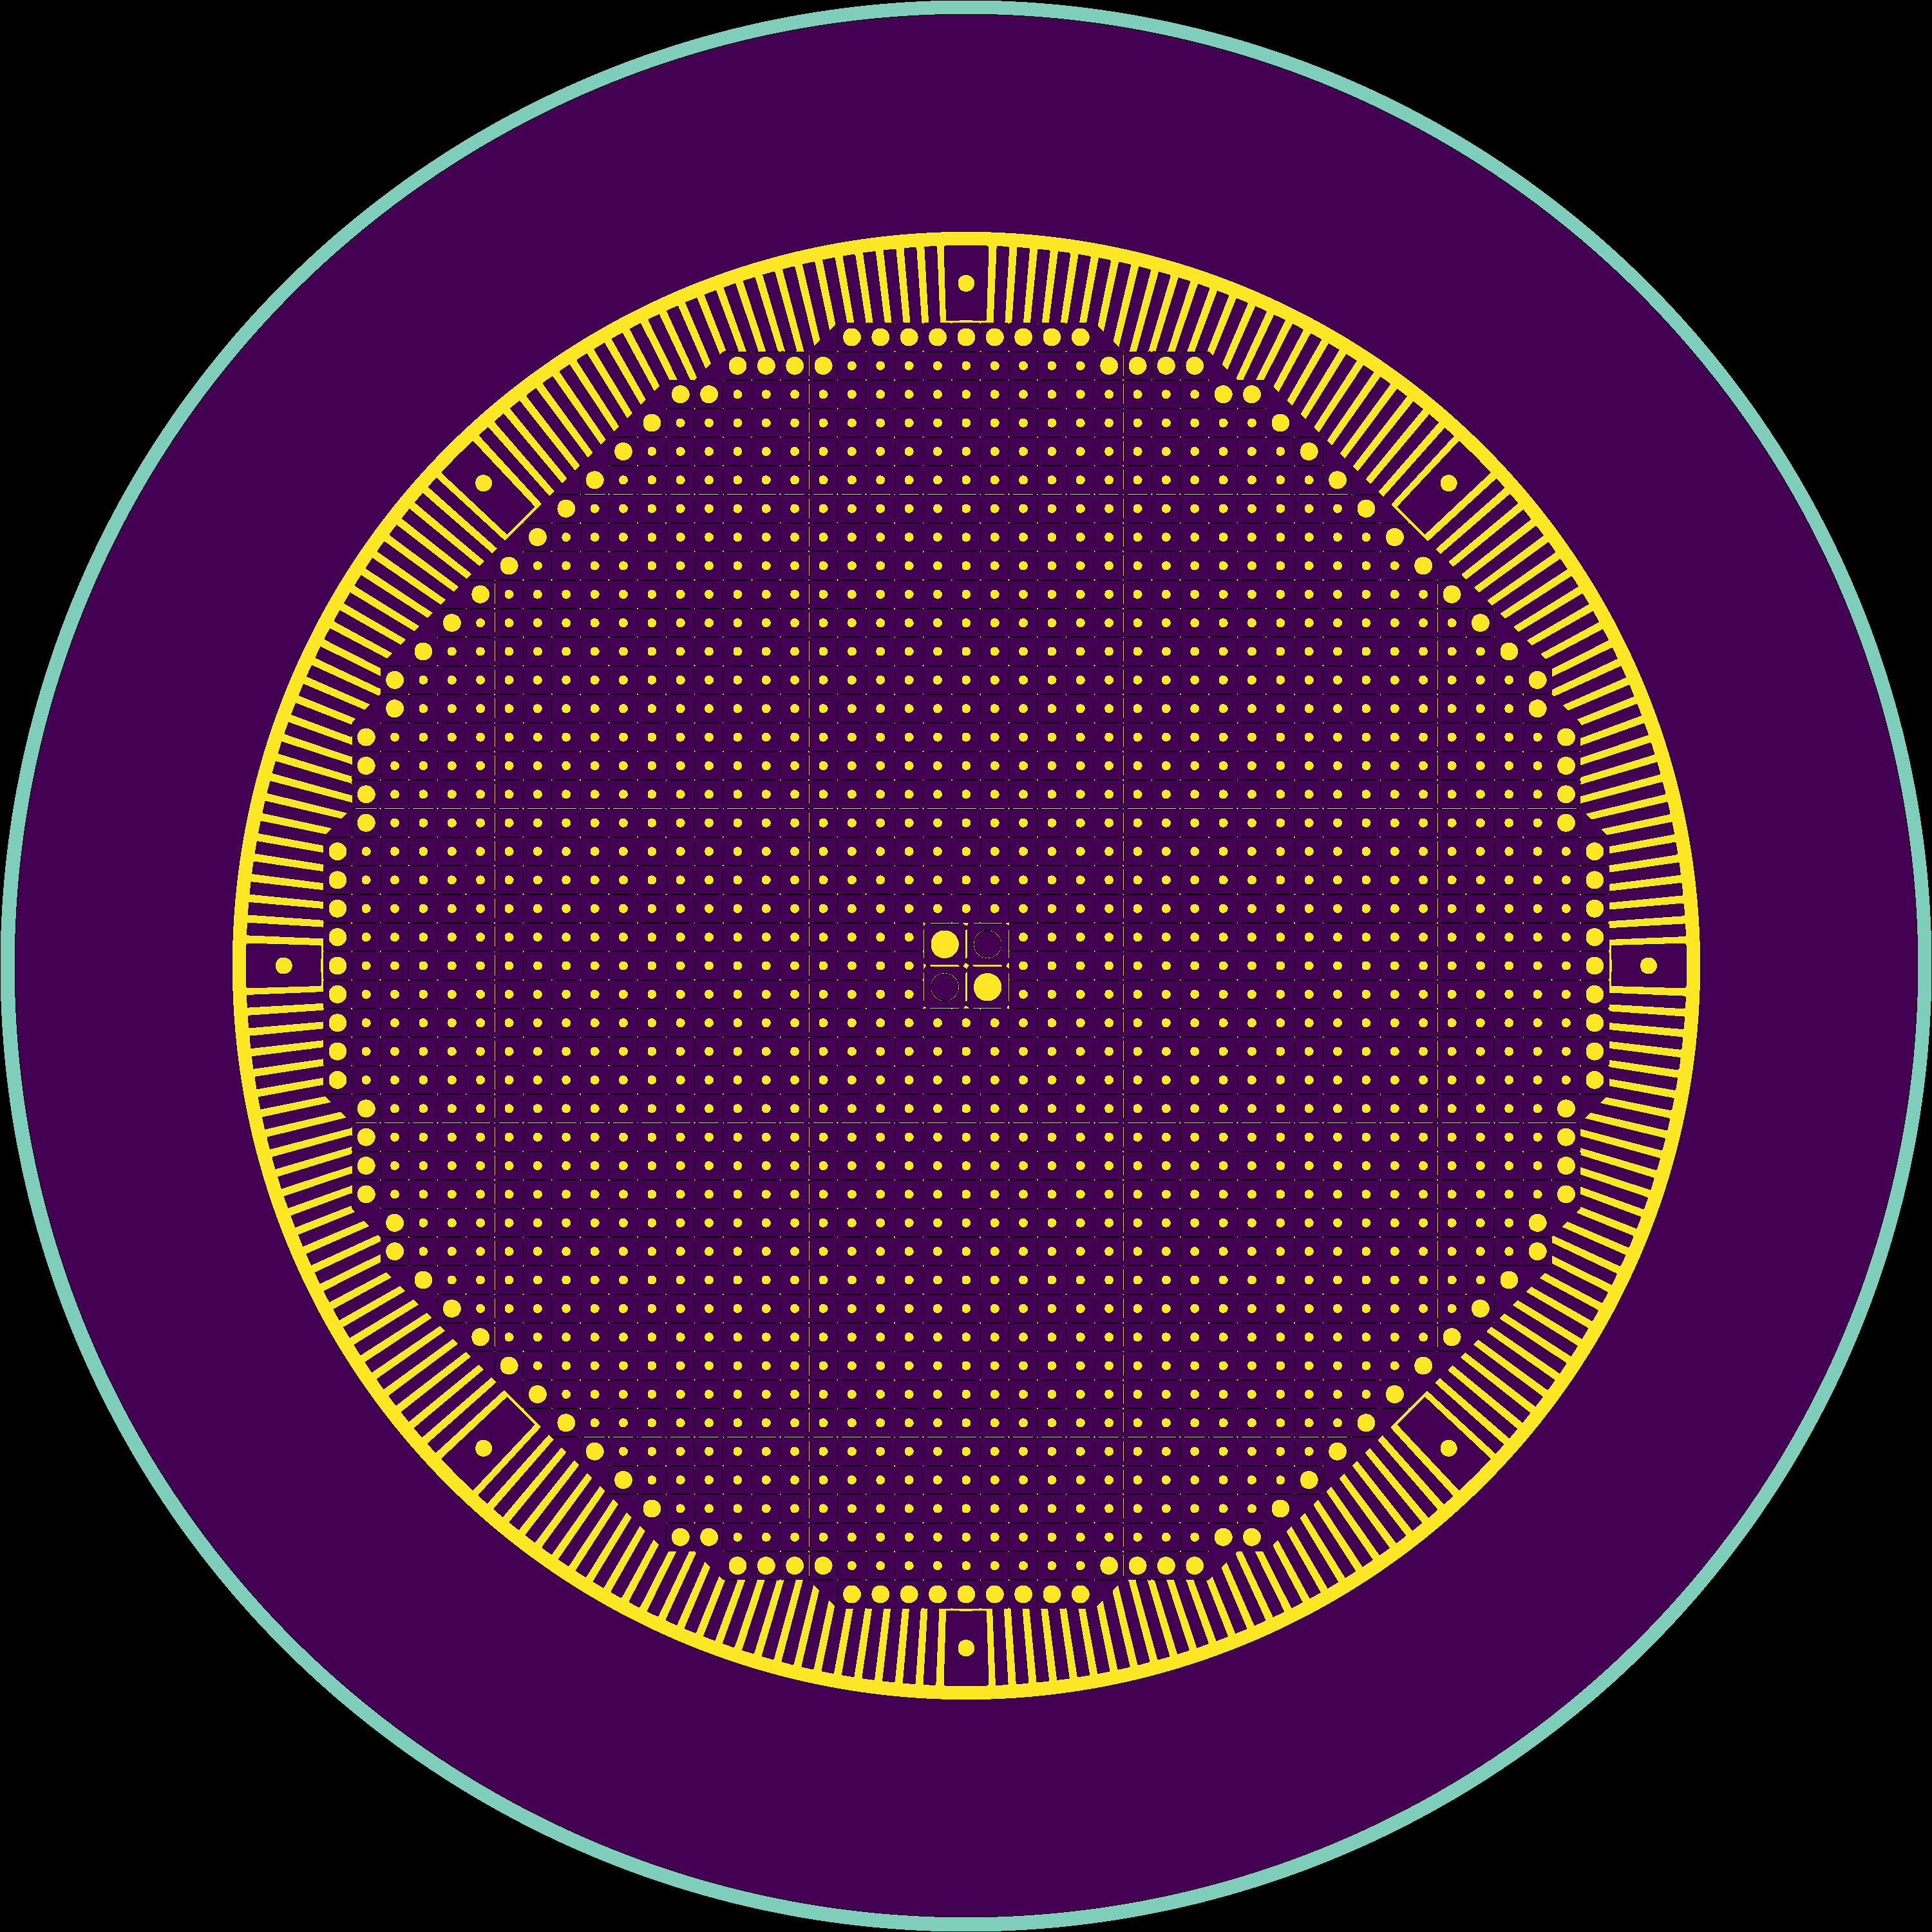
\includegraphics[width=0.95\linewidth]{figure_2_1.png}
  \caption{Plan view of \gls{MSBR} core.}
  \vspace{-0.6em}
  \label{fig:plan}
\end{figure}
\FloatBarrier

\begin{figure}[htbp!] % replace 't' with 'b' to force it to be on the bottom
  \centering
  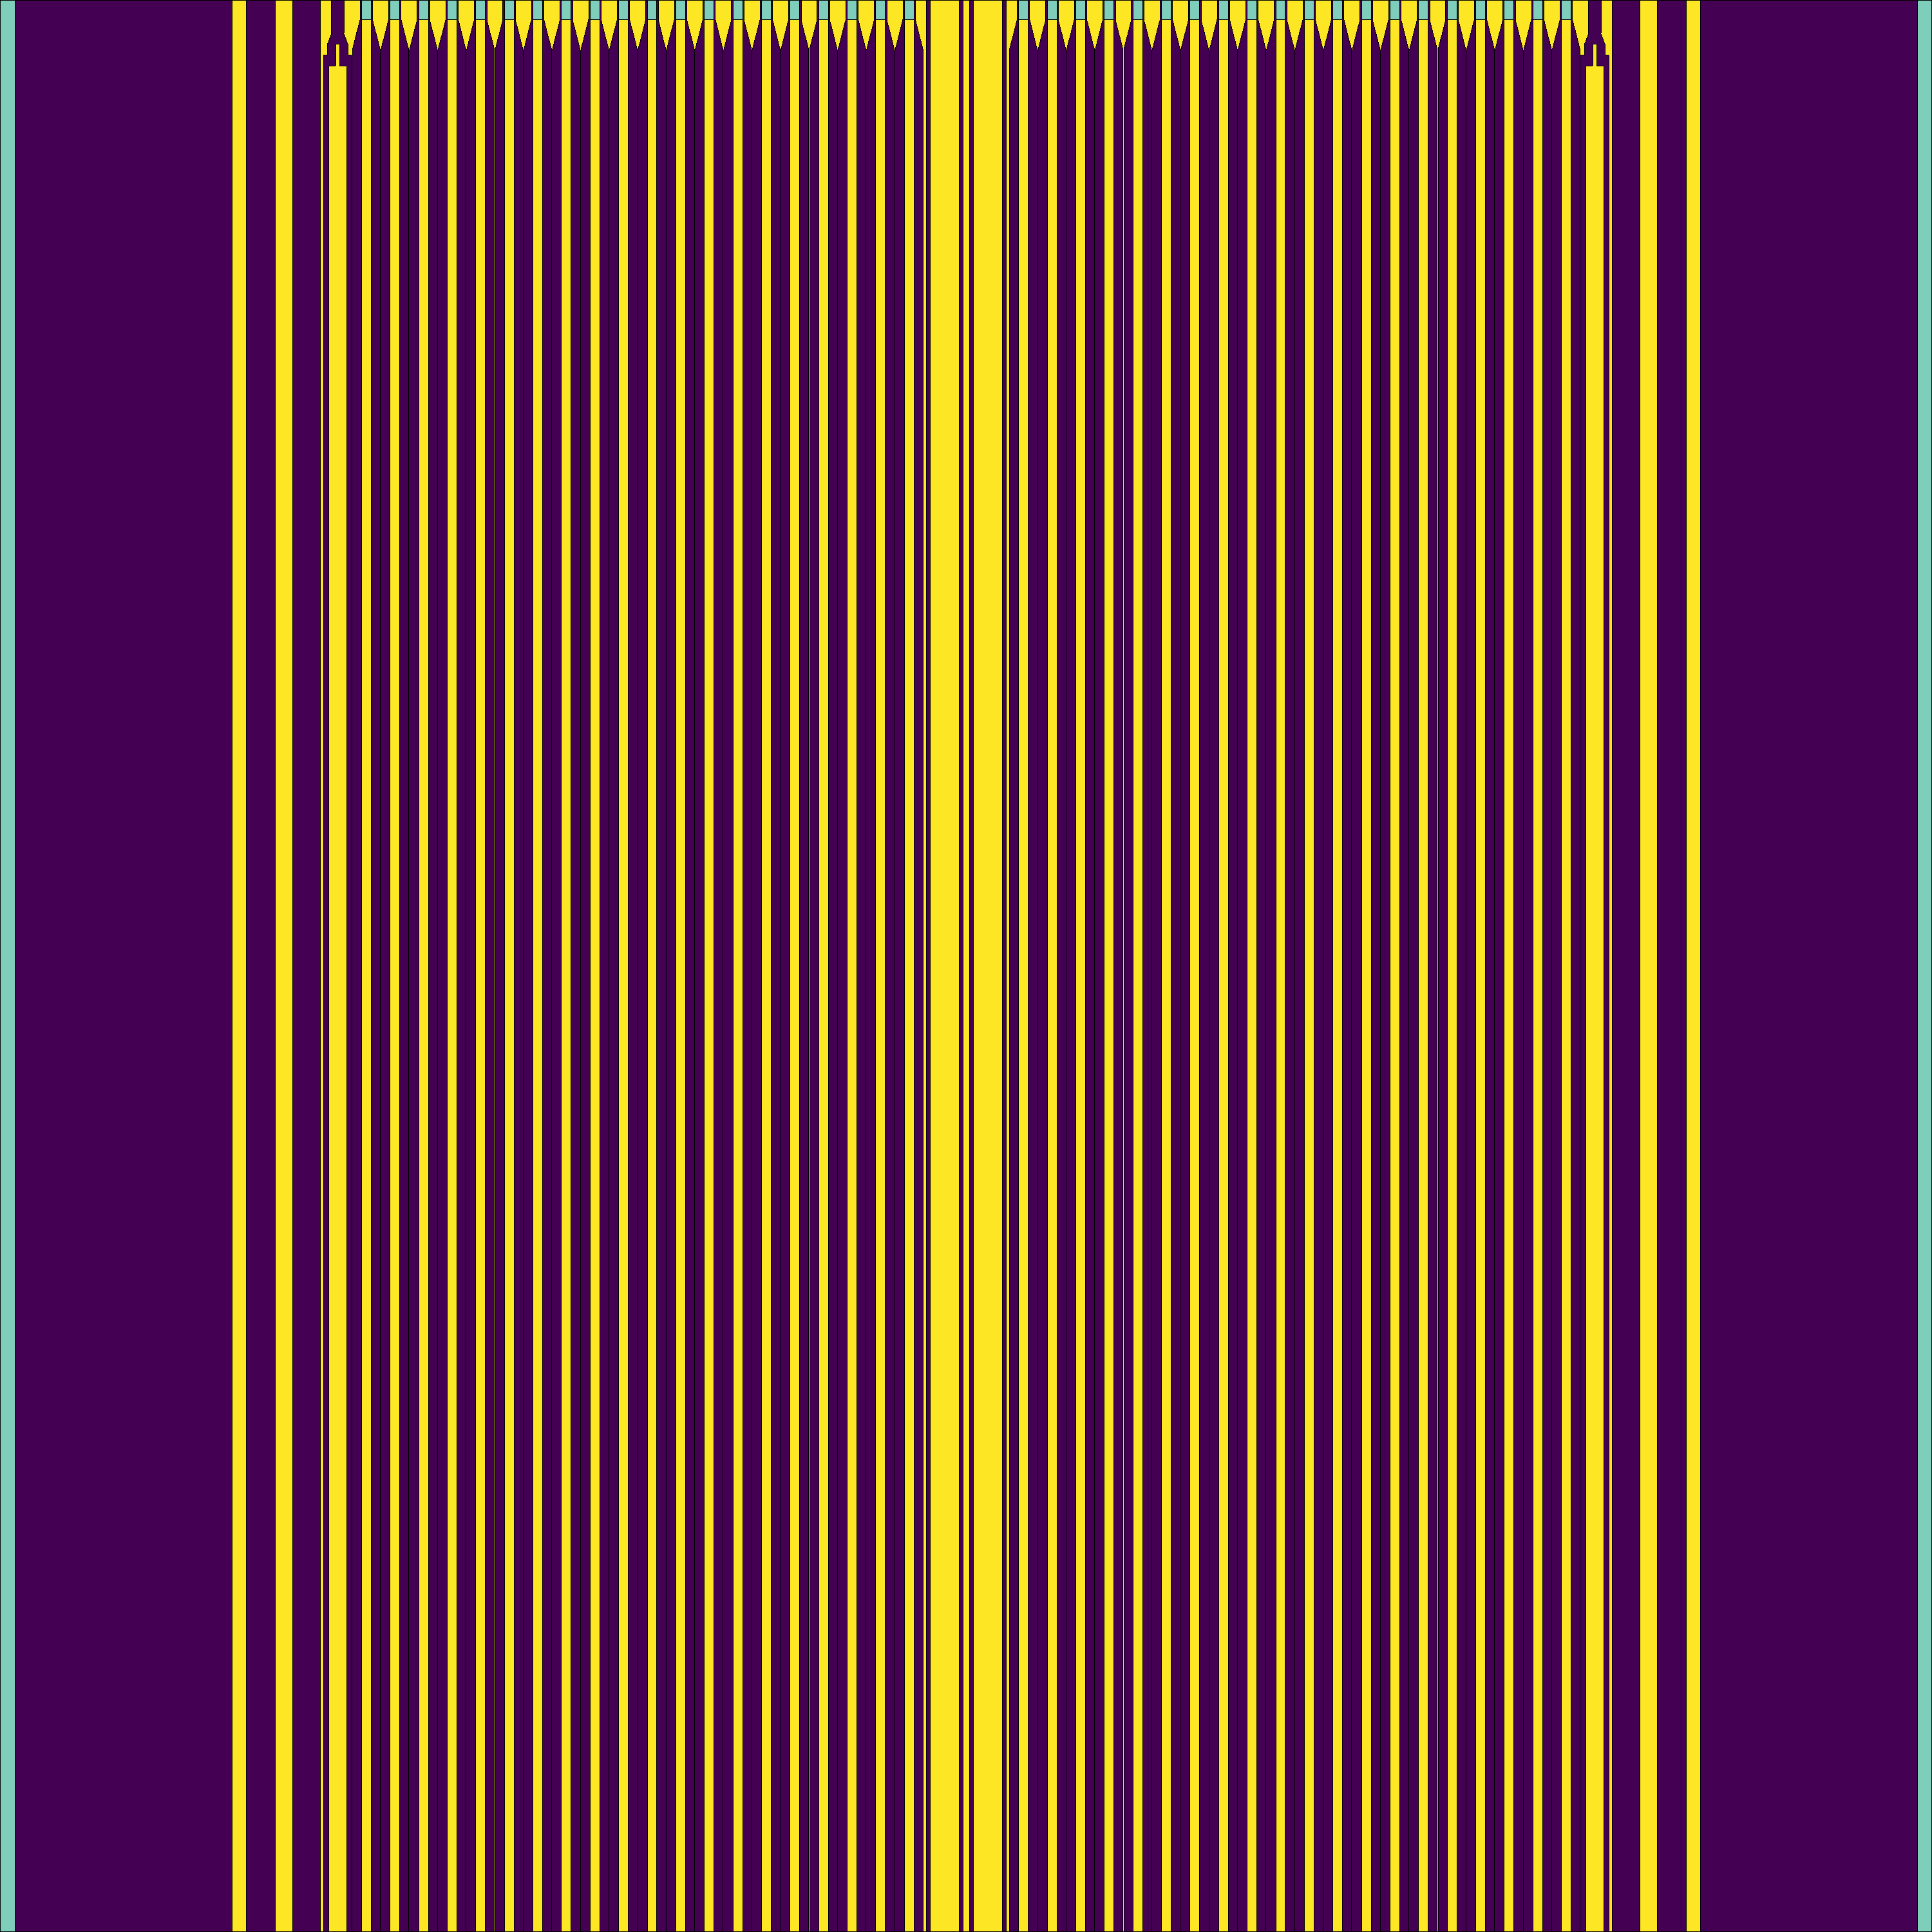
\includegraphics[width=\linewidth]{figure_2_2.png}
  \caption{Elevation view of \gls{MSBR} core.}
  \label{fig:elevation}
\end{figure}

\subsection{Core Zone I}

The central portion, called Zone I, is made up of 1320 graphite elements, each 
$10.16$cm$\times$10.16cm$\times$396.24cm.
In Zone I, 13\% of the volume is fuel salt and 87\% is graphite. Zone I is 
composed of 1320 graphite cells and 4 channels for control rods: two for 
graphite rods which both regulate and shim during normal operation, and two
for backup safety rods to assure sufficient negative reactivity for emergency 
situations.

These graphite elements have a mostly rectangular shape with lengthwise ridges 
at each corner that leave space for salt flow elements. Various element sizes 
reduce the peak damage flux and power density in the center of the core prevent 
local graphite damage. Figure~\ref{fig:zone12A} demonstrates the elevation and 
sectional views of graphite elements exactly as they are represented in this 
Monte Carlo model.

\subsection{Core Zone II}
The undermoderated zone, Zone II, surrounds Zone I.
Combined with the bounding radial reflector, Zone II serves to diminish neutron 
leakage. This zone is formed of two kinds of elements: elements like those in 
Zone I with a larger channel diameter (Zone II-A), and radial
graphite slats (Zone II-B). 

Zone II is Zone II 37\% salt by volume and each element has a fuel channel 
diameter of 6.604cm. It is divided into two different zones: Zone II-A and Zone 
II-B. The graphite elements for Zone II-A are prismatic. Zone II-B elements are 
rectangular slats spaced far enough apart to provide the 0.37 fuel salt volume 
fraction. Fig.~\ref{fig:zone2B} additionally shows the 5.08cm-wide annular 
space between the core graphite and the radial reflector graphite. The annulus 
contains 100\% fuel salt and serves to reduce the damage flux at the internal 
surface of the graphite reflector blocks. The reactor Zone II-B graphite 
5.08cm-thick slats vary in the radial dimension (average width is 26.67cm) but 
are reconstructed without any approximation. From the ORNL report 
\cite{robertson_conceptual_1971}, the suggested design of Zone II-B has 8 
irregularly-shaped graphite elements every 45$^\circ$ as well as salt channels. 
These graphite elements were simplified into right-circular cylindrical shapes 
with central channels. This is the only simplification made to the \gls{MSBR} 
conceptual geometry in this work.
\FloatBarrier
\begin{figure}[t] % replace 't' with 'b' to force it to be on the bottom
  \centering
  
\includegraphics[width=\linewidth]{figure_2_4.png}
  \caption{Zone I (left) and Zone II-A (right) elements.}
  \label{fig:zone12A}
\end{figure}
\FloatBarrier
\subsection{Material composition}
The fuel salt, the reactor graphite, and the modified HastelloyN are materials 
unique of the \gls{MSBR} and were created at \gls{ORNL}. The initial fuel salt 
loading composition is LiF-BeF$_2$-ThF$_4$-$^{233}$UF$_4$ (71.8-16-12-0.2 mole 
\%). The lithium in the molten salt fuel is a fully enriched $^{7}$Li because 
$^{6}$Li is a very strong neutron poison and becomes tritium upon neutron 
capture. For cross section generation, ENDF/B-VII was employed 
\cite{chadwick_endf/b-vii.0:_2006}. The specific temperature was fixed for each 
material to correctly model the Doppler-broadening of resonance peaks when 
Serpent generate problem-oriented nuclear data library.
%The isotope composition of each material at the initial state was described in 
%detail in the MSBR conceptual design study \cite{robertson_conceptual_1971} 
%and has been applied to Serpent model without any modification. %
\begin{figure}[htbp!] % replace 't' with 'b' to force it to be on the bottom
  \centering
  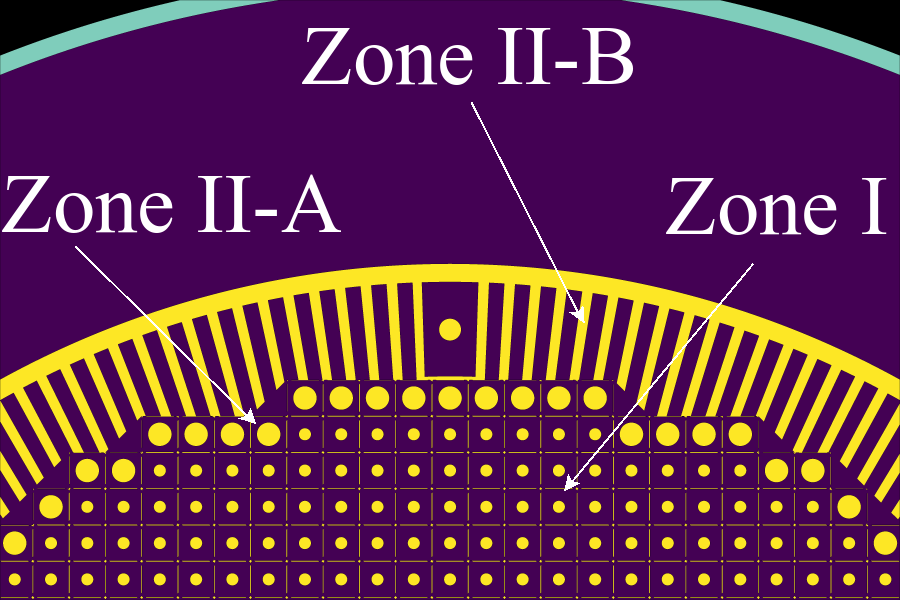
\includegraphics[width=0.89\linewidth]{figure_2_5.png}
  \caption{Plan view that includes Zone I, II-A, and II-B elements.}
    \vspace{-0.6em}
  \label{fig:zone2B}
\end{figure}
\FloatBarrier
%%%%%%%%%%%%%%%%%%%%%%%%%%%%%%%%%%%%%%%%%%%%%%%%%%%%%%%%%%%%%%%%%%%%%%%%%%%%%%%%
\section{Results}
This section presents calculation results, such as the effective multiplication 
factor for whole core, neutron flux spectrum, and temperature reactivity 
coefficients. The normalized neutron flux distribution is calculated for the 
whole core using continuous-energy nuclear data.
The temperature coefficients for both fuel salt solution and reactor graphite 
are computed by comparing effective multiplication factors for two temperatures 
in the working range.
 	
\subsection{Neutron spectrum}
Fig.~\ref{fig:spectrum} demonstrates the normalized neutron flux spectrum for 
the whole core in the energy range from $10^{-9}$ to $10$ MeV. The results show 
close fit with the MCNP simulation \cite{park_whole_2015}, especially in 
thermal energy range.  
\begin{figure}[b!] % replace 't' with 'b' to force it to 
  \centering
  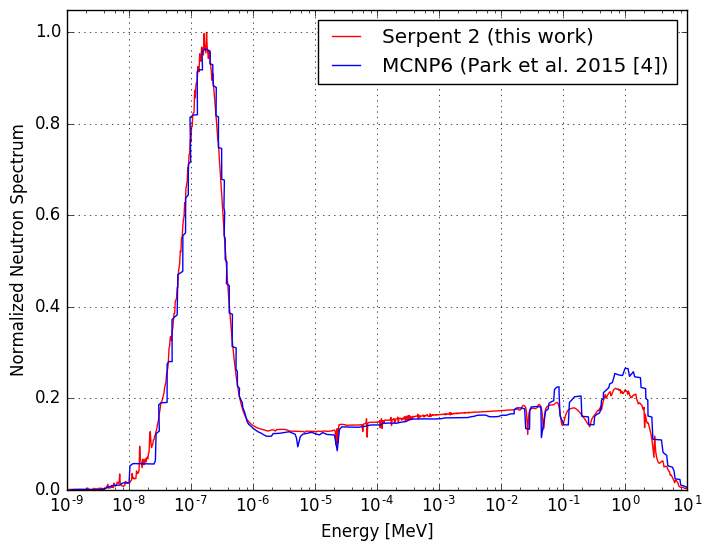
\includegraphics[width=1.05\linewidth]{figure_3_1.png} \caption{Neutron flux 
  spectrum of \gls{MSBR} for MCNP6 and Serpent 2 model.}
  \label{fig:spectrum}
\end{figure}
It is important to obtain the epithermal and thermal spectrum to produce 
$^{233}$U from $^{232}$Th because radiative capture cross section of thorium 
monotonically decreases from $10^{-10}$ MeV to $10^{-5}$ MeV. Hardening the 
spectrum tends to significantly increase resonance absorption in thorium and 
decrease the absorptions in fissile and construction materials. Thus, a 
signficant amount fissile material will be needed to make the reactor critical.

\subsection{Effective multiplication factor}
Table~\ref{tab:keff} shows the effective multiplication factor for both MCNP6 
and Serpent 2 whole core models. The factor obtained using Serpent 2 is 300 pcm 
lower than that obtained by Park \emph{et al.} using MCNP6 
\cite{park_whole_2015}. Standard deviations are 5 and 9 pcm, respectively. The 
discrepancy is likely due to simplificiations to the Zone II geometry model 
used in Park \emph{et al.}
%%%%%%%%%%%%%%%%%%%%%%%%%%%%%%%%%%%%%%%%
\captionsetup[table]{
  labelsep = newline,
  name = TABLE, justification=justified,
  singlelinecheck=false,%%%%%%% a single line is centered by default
  labelsep=colon,%%%%%%
  skip = \medskipamount}
\begin{table}[h!]
%\centering
\caption{Effective multiplication factor of whole core model.}
\begin{tabular}{p{0.15\linewidth} p{0.3\linewidth} p{0.3\linewidth}} \toprule
      & Serpent2      & MCNP6 \cite{park_whole_2015}          \\ \midrule
K$_{eff}$  & 1.00389$\pm$0.00005 & 1.00736$\pm$0.00009
\\
\bottomrule
\end{tabular}
  \label{tab:keff}
\end{table}
%%%%%%%%%%%%%%%%%%%%%%%%%%%%%%%%%%%%%%%%%%%%%%%%%%%%%%%%%%%%%%%%%%%%%%%%%%%%%%%%
\subsection{Temperature effect of reactivity}
Table~\ref{tab:tcoef} shows temperature effects on reactivity calculated in 
this work as compared to both \cite{park_whole_2015} and 
\cite{robertson_conceptual_1971}. Uncertainty for each temperature coefficient 
also appears in Table~\ref{tab:tcoef}. The main physical principle underlying 
the reactor temperature feedback is an expansion of matter when it is heated.  
When the fuel salt temperature increases, the density of the salt decreases, 
but at the same time, the total volume of fuel salt in the core remains 
constant because it is bounded by the graphite. When the reactor graphite 
temperature grows, the density of graphite declines creating additional space 
for fuel salt. To determine temperature coefficients, the cross-section 
temperatures for fuel and moderator were changed from 900K to 1200K. Three 
different cases were considered:
\begin{enumerate}  \item Temperature of fuel salt rising from 900K to 1200K.
\item Temperature of graphite rising from 900K to 1200K.  \item Whole reactor 
        temperature rising from 900K to 1200K.
\end{enumerate}

%%%%%%%%%%%%%%%%%%%%%%%%%%%%%%%%%%%%%%%%
\captionsetup[table]{
  labelsep = newline,
  name = TABLE, justification=justified,
  singlelinecheck=false,%%%%%%% a single line is centered by default
  labelsep=colon,%%%%%%
  skip = \medskipamount}
\begin{table}[h!]
%\centering
  \caption{Temperature coefficients of reactivity.}
\begin{tabular}{p{0.22\linewidth} p{0.22\linewidth} p{0.21\linewidth} 
        p{0.15\linewidth}} \toprule
   Reactivity coefficient [pcm/K]  & Serpent2      & MCNP6 
        \cite{park_whole_2015}   & Reference \cite{robertson_conceptual_1971}      
        \\ \midrule
Fuel salt        & $-3.70\pm0.016$ & $-3.20\pm0.05$ & $-3.22$ \\ \midrule
Moderator        & $+2.33\pm0.027$ & $-0.11\pm0.05$ & $+2.35$ \\ \midrule
Total            & $-1.57\pm0.033$ & $-3.21\pm0.04$ & $-0.87$ \\
\bottomrule
\end{tabular}
  \label{tab:tcoef}
\end{table}
%%%%%%%%%%%%%%%%%%%%%%%%%%%%%%%%%%%%%%%%%%%%%%%%%%%%%%%%%%%%%%%%%%%%%%%%%%%%%%%%
In the first case, changes in the fuel temperature only impact fuel density. In 
this case, the geometry is unchanged because fuel is a liquid. However, when 
the moderator heats up, both the density and the geometry change due to thermal 
expansion of the solid graphite blocks and reflector. Accordingly, the new 
graphite density was calculated using a linear temperature expansion 
coefficient of 1.3$\times10^{-6}$1/K \cite{robertson_conceptual_1971}. A new 
geometry input was created based on this information.

The fuel temperature coefficient (FTC) is negative due to thermal Doppler 
broadening of the resonance capture cross sections in the thorium and is in a 
good agreement with early research 
\cite{robertson_conceptual_1971,park_whole_2015}. The moderator temperature 
coefficient is positive due to changing density and would increase during 
reactor operation because of spectrum hardening along with fuel depletion 
\cite{park_whole_2015}. Finally, the total temperature coefficient of 
reactivity is relatively large and negative, despite graphite components, and 
affords excellent reactor stability and controllability.
%%%%%%%%%%%%%%%%%%%%%%%%%%%%%%%%%%%%%%%%%%%%%%%%%%%%%%%%%%%%%%%%%%%%%%%%%%%%%%%%
\section{Conclusions}
We performed \gls{MSBR} full-core analysis using the Serpent 2 Monte Carlo 
code. The complex geometry of the reactor is reconstructed in three-dimensional 
space without any major approximations. Accurate material data was employed to 
calculate reactor key design parameters. The effective multiplication factor 
for initial fuel composition is slightly higher than 1 (1.00389) which allows 
reactor operation from startup to the first online reprocessing cycle. The 
neutron flux energy spectrum was calculated for the whole core and represents 
the epithermal spectrum of the MSBR. The total temperature coefficient is 
negative, consequently, the MSBR has negative temperature feedback, but MTC is 
negative which has a negligible effect on safety because it is outweighed by 
the strong, negative FTC.

This high-fidelity full-core model will be employed for a number of future 
efforts. First, depletion simulation will be performed using Serpent 2 
depletion capabilities to find the equilibrium state of the MSBR, its optimal 
fuel salt composition, reprocessing characteristics (i.e. rates of removing 
fission products, the rate of adding thorium), and fuel utilization. Secondly, 
the model will be used to generate problem-oriented nuclear data libraries for 
multi-physics models of \glspl{MSR} developed in the MOOSE-based coupled 
neutronics/thermal-hydraulics code Moltres \cite{lindsay_arfc/moltres:_2017}.  
Finally, transient accident simulations for safety investigation of the reactor 
core will be performed to study the dynamic behavior of Molten Salt Breeder 
Reactor. 


%%%%%%%%%%%%%%%%%%%%%%%%%%%%%%%%%%%%%%%%%%%%%%%%%%%%%%%%%%%%%%%%%%%%%%%%%%%%%%%%
\bibliographystyle{ans}
\bibliography{bibliography}
\end{document}

